%!TEX root = ../dissertation.tex
%\begin{savequote}[75mm]
%Nulla facilisi. In vel sem. Morbi id urna in diam %dignissim feugiat. Proin molestie tortor eu velit. %Aliquam erat volutpat. Nullam ultrices, diam tempus %vulputate egestas, eros pede varius leo.
%\qauthor{Quoteauthor Lastname}
%\end{savequote}

\chapter{Algoritmos implementados}

%\newthought{There's something to be said}
En este capítulo se revisan los seis algoritmos de preprocesamiento y clasificación de datos ordinales y monotónicos implementados en el paquete software desarrollado, ofreciendo una descripción teórica de los mismos. Para ello se divide el capítutlo en dos secciones: algoritmos de preprocesamiento y algoritmos de clasificación.
\section{Preprocesamiento}
\subsection{Selector de características para clasificación monotónica}
Se implementa en el paquete el algoritmo para selección de características \cite{hu2012feature} basado en Rank Mutual Information. El funcionamiento del algoritmo propuesto por Qinghua Hu et Al. es el siguiente: \newline
 Consideremos un conjunto de datos $\langle U, A, D \rangle$ donde $U$ denota las instancias, $A$ denota los atributos y $D$ las clases, tal que $D=d_1 < d_2 < ... < d_k$. Entonces, para cada atributo $a \in A$ se calculan las relaciones entre las instancias usando la siguiente función \textit{logsig}: 
 $$r_{ij}^{<}=\frac{1}{1+e^{\ k \ ( v(x_i,a)-v(x_j,a) )}}$$
 Donde $v(x_i,a)$ es el valor de la instancia $x_i$ para el atributo $a$, y $k$ es una constante positiva.
 El resultado de aplicar esta función es:
 
\[ 
\left \{
\begin{tabular}{cc}
0.5, & si $r_{ii}^{>}=r_{ii}^{<}$ \\
$\approx 1$, & si $v(x_j,a) >> v(x_i,a)$  \\
$\approx 0$, & si $v(x_j,a) << v(x_i,a)$ 
\end{tabular}
\right \}
\]

Es decir, en el primer caso no habría diferencia entre $x_i$ y $x_j$, en el segundo caso $x_i$ sería significativamente inferior a $x_j$, y en el tercer caso $x_i$ sería significativamente mayor. \newline
Con esto se calculan los conjuntos ordinales difusos mayores que $x_i$ en términos de $a$ de la siguiente forma:
$$[x_i]_a^{\leq}=r_{i1}/x_1 + r_{i2}/x_2 +...+r_{in}/x_n$$
que serán posteriormente usados para calcular la \textit{mutual rank information} entre dos atributos cualesquiera sobre un conjunto de instancias de la siguiente forma: 
$$RMI_{a_1,a_2}(U)= -\sum_{i=1}^{n} \frac{1}{n} \log \frac{| [x_i]_{a_1}^{\leq}| \times |[x_i]_{a_2}^{\leq}|  }{ n \times | [x_i]_{a_1}^{\leq} \cap [x_i]_{a_2}^{\leq} |}$$

Esta ganancia de información se combina junto con la ganancia de información de cada característica con respecto a la clase, obteniendo el criterio mRMR (minimum redundancy maximum relevance), que trata de encontrar las características más significativas y menos relevantes:
$$\Phi=\frac{1}{|B|} \sum_{a_i \in B} RMI_{a_i,D} - \frac{\beta}{|B|^2} \sum_{a_i, a_j \in B} RMI_{a_i,a_j} $$ 
donde $\beta$ es un parámetro regulativo. Finalmente se seleccionan las \textit{$k$} características con mayor mRMR.
\subsection{Selector de instancias para clasificación monotónica}
EL selector de instancias para datos monotónicos implementado en el paquete es el algoritmo propuesto por J.-R. Cano, S. García, de nombre MonTSS \cite{cano2017training}. \newline
 MonTSS tiene como objetivo eliminar las instancias que no son interesantes para el problema monotónico, lo que reduce la dimensión del problema y, como efecto colateral, los costes de computación. El algoritmo se compone de tres fases, como ilustra la siguiente figura:
 \begin{figure}[h]
 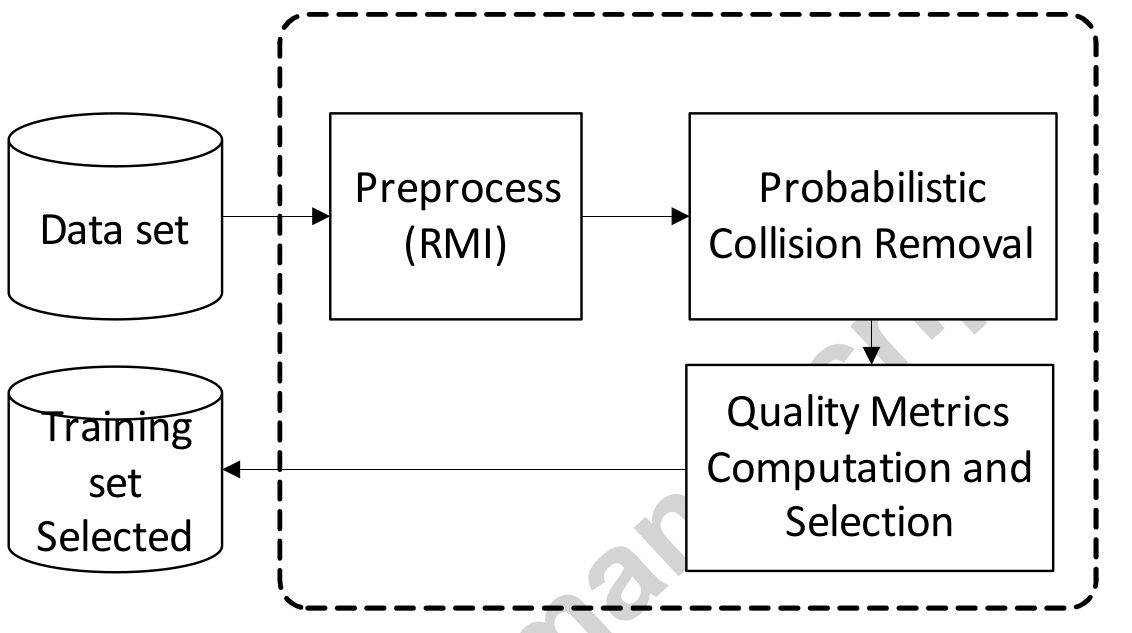
\includegraphics[width=\textwidth]{figures/montss}
 \caption[Short figure name.]{Fases del proceso de MonTSS.
\label{fig:myInlineFigure}}
 \end{figure}

\begin{itemize}
	\item \textbf{Preprocesamiento}: se analiza inicialmente la relación de cada característica con la clase, usando RMI de forma similar a la descrita en el algoritmo anterior. Las características seleccionadas en este paso serán las empleadas en pasos posteriores del algoritmo.
	\item \textbf{Eliminación de colisiones}: se trata de un proceso iterativo en el que se eliminan la mayoría de las instancias que producen colisiones, es decir, las que no son monótonas. Para ello se comienza calculando el número de colisiones que produce cada instancia, tras lo que se ordenan de forma decreciente. Luego se emplean la tasa de candidatos a seleccionar y el número de colisiones permitidas especificadas previamente al algoritmo como parámetro, para eliminar las instancias. Este último paso se hace de forma probabilística, pues para seleccionar la instancia a eliminar se genera un valor entre $\left[1,maxCandidates \right]$, Donde \textit{maxCandidates} se calcula a partir del tamaño de los datos y de la tasa de candidatos. El proceso se repite hasta que se alcanza el número permitido de colisiones.
	\item \textbf{Cálculo de métricas}: de entre las instancias seleccionadas en el paso anterior, se seleccionan finalmente las más importantes, que son las que se corresponden con fronteras de decisión. Para detectarlas, se emplean dos métricas, llamadas \textit{Delimitación} e \textit{Influencia}. Se calculan como sigue:
	$$Del(x_i)=\frac{|Dom(x_i)-NoDom(x_i)|}{Dom(x_i)+NoDom(x_i)}$$
	Donde $$Dom(x_i)=x' \in X' \iff x_i \prec x' \land Y(x_i)=Y(x')$$
	$$NoDom(x_i)=x' \in Z' \iff x_i \succeq x' \land Y(x_i)=Y(x')$$
	Es decir, $Dom(x_i)$ son las instancias con igual clase que $x_i$ que dominan a ésta, mientras que $NoDom(x_i)$ son las instancias con igual clase a $x_i$ que son dominadas por ella. \newline
	Por otro lado, la influencia de una instancia $x_i$ se calcula empleando los vecinos con diferente clase y su distancia a $x_i$, que se traduce en un peso asociado: 
	$$Infl(x_i)=\sum_{j=1}^{k} influenceWeight(x_j)$$
	donde $influenceWeight$ se calcula como el peso normalizado de la instancia $x_j$ y se cumple que $Y(x_i) \neq Y(x_j) \land x_j \in kNN_{xi}$. \newline
	Ambas métricas toman valores en el rango $\left[0,1\right]$, considerando 1 como muy relevante. 
\end{itemize}
\section{Clasificación}
\subsection{SVMOP}
Se implementa el ensemble de WSVMs para clasificación ordinal \cite{waegeman2009ensemble} usando descomposición binaria.
Esta técnica se basa en descomponer el problema en varios subproblemas binarios, entrenando $r-1$ SVM's, donde $r$ denota el número de clases del problema. 
Sigue un enfoque muy similar al de emsembles probabilísticos que propuso Frank \& Hall \cite{frank2001simple}:

\begin{figure}[H]
	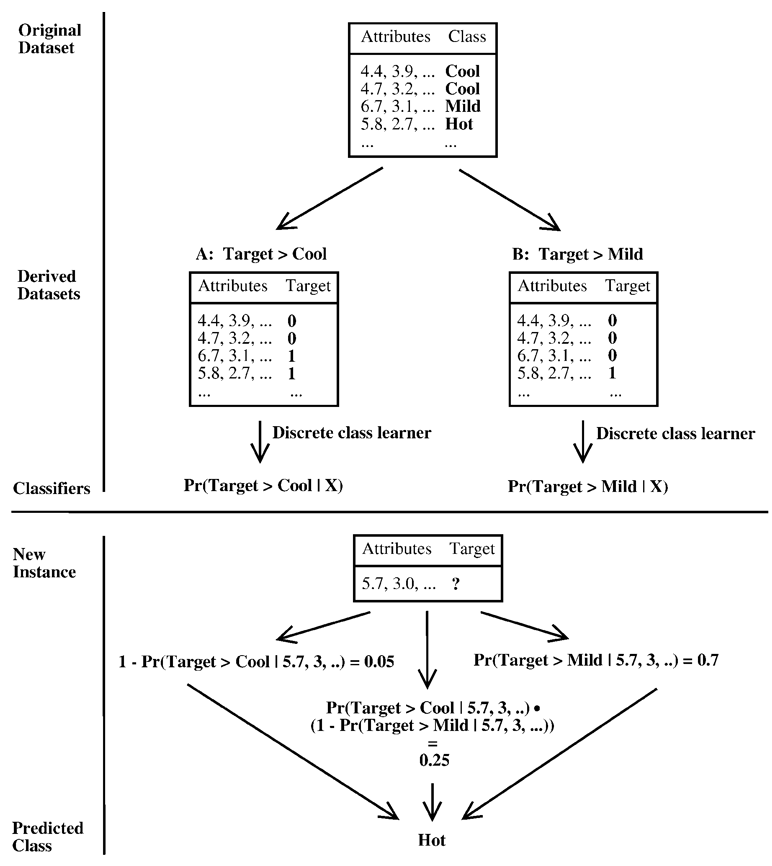
\includegraphics[width=\textwidth]{figures/Frankhall}
	\caption[Short figure name.]{Aplicando algoritmos de clasificación estándar a predicción ordinal.
		\label{fig:myInlineFigure}}
\end{figure}



En concreto, para cada clasificador binario se transforman las instancias de entrenamiento a la clase positiva o negativa, binarizándolas en función de si su etiqueta es mayor o no que $p$, donde $p=1,...,r-1$. \newline
\[ 
y_{pi}=
\left \{
\begin{tabular}{cc}
-1, & si $y_i \leq p$ \\
1, & si $y_i > p$  
\end{tabular}
\right \}
\]

Siguiendo con el enfoque Frank \& Hall, tras esto hay que asignarle un peso a cada una de las muestras, que será diferente para cada clasificador, lo que implica resolver los $r-1$ problemas de optimización subyacentes. \newline
Los pesos se asignan de forma que los errores de clasificación sean penalizados proporcionalmente a la diferencia absoluta de la clase de la instancia y $p$:
\[ 
v_{pi}=
\left \{
\begin{tabular}{cc}
$(p + 1 -y_i) \frac{| \left\{ x_i | y_i \leq p \right\} |}{\sum_{i=1;y_i \leq p }^{n}(p+1 -y_i)}$, & si $y_i \leq p$ \\
$(y_i -p)\frac{| \left\{ x_i | y_i > p \right\} |}{\sum_{i=1;y_i > p }^{n}(y_i -p)}$, & si $y_i > p$  
\end{tabular}
\right \}
\]

y se escalan para que mantenga igual la suma de errores de las clases positiva y negativa. Las clases de los datos de test se estiman combinando las $\hat{y}_{pi}$ predicciones obtenidas por los $r-1$ clasificadores, de tal forma que asignaremos la clase $k$ a $x_i$ si $\hat{y}_{pi}=1$ para todo $p < (k-1)$ y $\hat{y}_{pi}=-1$ para todo $p \geq k$. Sin embargo, para problemas multiclase a menudo ocurren ambigüedades con este proceso de asignación de clase, por lo que se asigna la clase con mayor probabilidad. En la implementación se usa \textit{libsvm-weights} \cite{chang2011libsvm} para el entrenamiento de las SVMs.
\subsection{POM}
Se implementa el modelo linear de regresión \textit{Proportional Odd Model for Ordinal Regression} \cite{mccullagh1980regression} como un modelo de regresión logística, en base a lo siguiente:\newline
Sean $k$ las categorías ordenadas de la variable de clase, con probabilidades $\pi_1(x),\pi_2(x),...,\pi_k(x)$ donde las variables observadas toman valor $x$. En el caso de que hubiera dos grupos, $x$ sería una variable factor que indicaría la pertenencia a cada grupo. Sea $Y$ la variable de clase que toma valores en el intervalo $\left[1,...,k\right]$ con las probabilidades mencionadas arriba, y sea $k_j(x)$ la cuota de que $Y \leq j$ dado $x$. Entonces el modelo POM especifica que:
$$k_j(x)=k_j \exp (-\beta^T x), (1 \leq j < k)$$ 
Donde $\beta$ es un vector de parámetros desconocidos. El ratio de las cuotas correspondientes se calcula como:
$$k_j(x_1)/k_j(x_2)= \exp \left\{ \beta^T (x_2 - x_1)\right\}, (1 \leq j < k)$$
y es independiente de $j$, dependiendo únicamente de la diferencia de las covariables $x_2,x_1$. Entonces, como la cuota de $Y \leq j$ es el ratio $\gamma_j(x)/ \left\{ 1- \gamma_j(x) \right\}$, donde $\gamma_j(x)=\pi_1(x)+...+\pi_j(x)$, el modelo POM resulta idéntico a el modelo de regresión logística lineal:
$$\log \left[ \gamma_j(x)/ \left\{ 1- \gamma_j(x) \right\} \right] = \theta_j - \beta^T x , (1 \leq j < k)$$

donde $\theta_j=\log(k_j)$ por lo que la diferencia entre logits comulativos es independiente de la categoría.

\subsection{KDLOR}
\textit{Kernel Discriminant Learning for Ordinal Regression}  \cite{sun2010kernel}
\subsection{WKNN}
Se implementa la extensión de KNN para datos ordinales 
\textit{Weighted k-Nearest-Neighbors} \cite{hechenbichler2004weighted} que se basa en la idea de que las observaciones del conjunto de entrenamiento más próximas a la nueva observación a clasificar deben tener un mayor peso en su decisión. Además, para que el algoritmo sea también aplicable a datos monotónicos, se le incorporan restricciones de monotonicidad \cite{duivesteijn2008nearest}.

El procedimiento del algoritmo se puede describir como:
\begin{enumerate}
	\item \textbf{Estandarización de variables}: previamente al cálculo de las distancias, para lo que se divide cada variable por su desviación estándar.
	\item \textbf{Obtención de vecinos}: Sea $L= \left\{ (y_i,x_i), i=1,...,n_L \right\}$ un conjunto de entrenamiento donde $x_i$ denota la instancia e $y_i$ denota la clase. Dada una nueva instancia de test $x$ a clasificar, se obtienen sus $k+1$ vecinos más cercanos de acuerdo a la distancia de Minkowski, dado el parámetro $q$ de la misma.
	\item \textbf{Estandarización por el (k+1)ésimo vecino}: se estandarizan las $k$ distancias obtenidas en el paso anterior usando el vecino $k+1$ que no será considerado para la clasificación de  $x$, tal que:
	$$D_{(i)}=D(x,x_{(i)})= \frac{d(x,x_{(i)})}{d(x,x_{k+1})}$$
	\item \textbf{Asignación de pesos:} se transforman las distancias $D_{(i)}$ normalizadas a pesos, usando para ello alguna de las funciones Kernel implementadas, tal que $w_{(i)}=K(D_{(i)})$. Los Kernels que se implementan son: 
	\begin{itemize}
		\item Rectangular: $\frac{1}{2} \cdot I(|d|\leq 1)$
		\item Triangular: $(1 - |d|) \cdot I(|d| \leq 1)$
		\item Epanechnikov: $\frac{3}{4}(1 - d^2) \cdot I(|d| \leq 1)$
		\item Biweight: $\frac{15}{16} (1 - d^2)^2 \cdot I(|d| \leq 1)$
		\item Triweight: $\frac{35}{32} (1-d^2)^3 \cdot I(|d| \leq 1)$
		\item Coseno: $\frac{\pi}{4} \cos(\frac{\pi}{2}d) \cdot I(|d| \leq 1)$
		\item Gaussiano: $\frac{1}{\sqrt{2 \pi}} \exp(- \frac{d^2}{2})$
		\item Inversión: $\frac{1}{|d|}$
	\end{itemize}
		\item  \textbf{Asignación de clase}: por último, se etiqueta $x$ con clase $y$ donde $y$ es la clase con mayor peso de entre sus vecinos.
\end{enumerate}

Si se especifica el parámetro de monotonía, entonces se aplican restricciones monotónicas en la asignación de clases, de tal forma que se restinge la clase que puede tomar una instancia al intervalo $\left[y_{min},y_{max}\right]$, donde:
$$y_{min}=\max \left\{ y | (x',y) \in D \land x' \leq x \right\}}$$
y
$$y_{max}=\min \left\{ y | (x',y) \in D \land x \leq x' \right\}}$$

Por tanto el procedimiento es el mismo que el anterior pero, en este caso, al obtener los $k$ vecinos de la nueva instancia a clasificar, $x$, le asignamos la etiqueta de sus vecinos más frecuente que se encuentre en el intervalo $\left[y_{min},y_{max}\right]$. Si ninguna etiqueta se encuentra en ese indervalo, se le asigna una aleatoria del intervalo.
%% Requires fltpage2 package
%%
% \begin{FPfigure}
% 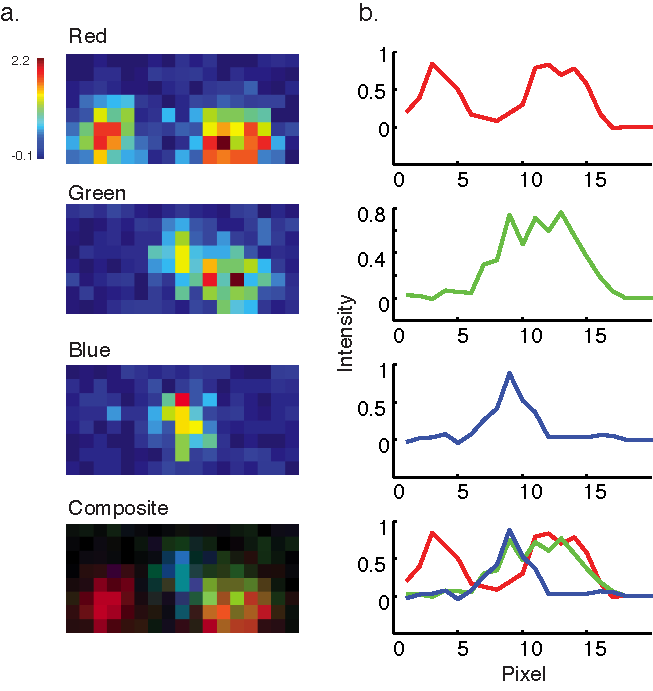
\includegraphics[width=\textwidth]{figures/fullpage}
% \caption[Short figure name.]{This is a full page figure using the FPfigure command. It takes up the whole page and the caption appears on the preceding page. Its useful for large figures. Harvard's rules about full page figures are tricky, but you don't have to worry about it because we took care of it for you. For example, the full figure is supposed to have a title in the same style as the caption but without the actual caption. The caption is supposed to appear alone on the preceding page with no other text. You do't have to worry about any of that. We have modified the fltpage package to make it work. This is a lengthy caption and it clearly would not fit on the same page as the figure. Note that you should only use the FPfigure command in instances where the figure really is too large. If the figure is small enough to fit by the caption than it does not produce the desired effect. Good luck with your thesis. I have to keep writing this to make the caption really long. LaTex is a lot of fun. You will enjoy working with it. Good luck on your post doctoral life! I am looking forward to mine. \label{fig:myFullPageFigure}}
% \end{FPfigure}
% \afterpage{\clearpage}
